\documentclass[12pt]{article} 

\usepackage[latin1]{inputenc}
\usepackage[spanish]{babel}
\usepackage{color}
\usepackage{multicol}
\usepackage{amsmath}
\usepackage{amssymb}
\usepackage{enumerate}
\usepackage{graphics}
\usepackage{graphicx}

\title{BICOLOREAR}
\author{Sara Chica, Rodrigo Gualtero}
\date{29 de Septiembre, 2012}

\begin{document}
\maketitle
\tableofcontents

\section{Introducci�n}
Este es un problema de la UVA, identificado con el c�digo \textit{10004}, en el cual se desea saber si un grafo ingresado es o no bicoloreable.
\\Un Grafo es \textit{bicoloreable} si se pueden pintar todos sus nodos solamente con dos colores, es decir, si no existen dos nodos adyacentes con el mismo color; en caso contrario, es un nodo \textit{No Bicoloreable}.
\\A continuaci�n se presentan 2 ejemplos de nodos:

\begin{center}
	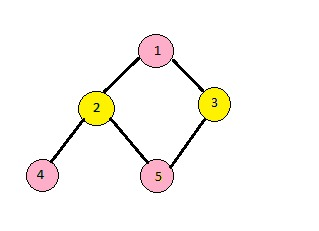
\includegraphics[width=0.50\textwidth]{Bicoloreable.jpg}
	\\Ejemplo 1: Nodo Bicoloreable
\end{center}

\begin{center}
	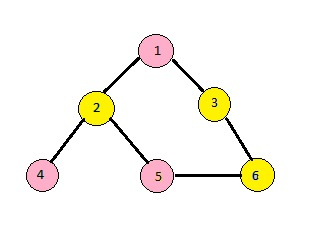
\includegraphics[width=0.50\textwidth]{NoBicoloreable.jpg}
	\\Ejemplo 2: Nodo No Bicoloreable
\end{center}

\section{Definici�n del problema}
Para este problema se suponen 3 cosas:
\begin{enumerate}
	\item Un nodo no tiene una conexi�n consigo mismo.
	\item El grafo es no dirigido, es decir que, para todos los nodos, si \textit{a} est� conectado con \textit{b}, no necesariamente implica que \textit{b} lo est� con \textit{a}.
	\item El grafo es conexo.
\end{enumerate}
\subsection{Entrada}
Como primer lugar entra un valor que determina el n�mero de nodos, este debe ser entre 0 y 200.
\\Seguido a esto entra un n�mero, el cual indica la cantidad de conexiones.
\\Finalmente entran todas las conexiones con formato <<a b>>.
\subsection{Salida}
Si es bicoloreable imprime <<Bicoloreable>>, de lo contrario, imprime <<No bicoloreable>>.
\section{Modelamiento matem�tico}
Sea G un grafo, $G(V,L)$, donde
\\
\\V es el conjunto de nodos del grafo, 
\[ V=\left\{ a_{1}, a_{2}, ... , a_{n} \right\}  \]
\\y L es el conjunto de todas las conexiones, 
\[ L= \left\{(a_{1},a_{2}),(a_{1},a_{3}), ... , (a_{1},a_{n}), (a_{2},a_{3}), (a_{2},a_{4}), ... , (a_{n-1},a_{n})\right\} \]
\\El grafo es conexo si, para un par de nodos del grafo, existe una sucesi�n de arcos que permitan ir de uno a otro y devolverse.
\\El grafo es no dirigido si $(a,b)\Rightarrow(b,a)$.
\\No existe una conexi�n tal que $(a,a)$; es decir $(a,a) \notin L$
\\
\\Una matriz de adyacencia es una matriz cuadrada que se utiliza para representar las conexiones de un grafo, en donde 0 implica que no hay ninguna conexi�n, y 1 implica que existe una conexi�n. 
La matriz para este ejercicio cumple con las siguientes propiedades:
\begin{enumerate}
	\item Es sim�trica, por lo tanto es igual a su transpuesta, $M^{T}=M$; es decir, que
		\[
			(\forall _{i,j} | 0 \leq i \leq n \wedge 0 \leq j \leq n \wedge i \neq j: M_{ij} = M_{ji})
		\]
	\item Todos los elementos de su diagonal principal son 0, ya que ning�n nodo de la matriz tiene conexi�n consigo mismo,
		\[
			(\forall _{i,j} | i = j: M_{ij}=0)
		\]
\end{enumerate}
Utilizando el gr�fico del \textit{ejemplo 1} , se tiene la siguiente matriz de adyacencia:
 
\[
\begin{bmatrix}
0&1&1&0&0\\
1&0&0&1&1\\
1&0&0&0&1\\
0&1&0&0&0\\
0&1&1&0&0
\end{bmatrix}
\]

\section{Planteamiento de la Soluci�n}
Para determinar la soluci�n del problema se debe saber que un nodo es no bicoloreable siempre y cuando 2 nodos adyacentes a el tienen diferente color.
\[
NoBicoloreable \equiv (\exists a,b,c | a,b,c \in V : (a,b) \wedge (b,c) \wedge (a,c) )
\]
\\Es decir si un nodo \textit{a} tiene como nodos adyacentes \textit{b} y \textit{c}, donde \textit{b} es azul y \textit{c} rojo, entonces autom�ticamente el grafo es no bicoloreable, ya que \textit{a}, con cualquier color que tome, queda con el mismo color de alguno de sus nodos adyacentes.
\\Para solucionar el problema es importante tener en cuenta que se usa una matriz de adyacencia para saber las diferentes conexiones que existen, adem�s de esto a medida que se va llenando la matriz con las diferentes conexiones que entran se le va asignando color a los nodos, revisando sus nodos adyacentes, de esta forma en caso de que estos tengan diferentes colores se sabe que el nodo es no bicoloreable.
\section{Conclusiones}
\begin{enumerate}
	\item La mejor manera de modelar el grafo en este caso es una matriz de adyacencia, ya que teniendo las conexiones almacenadas se logra de manera m�s eficientes saber cuales nodos son o no bicoloreables.
	\item Se hace m�s eficiente la soluci�n si a medida que se van ingresando las diferentes conexiones se va mirando si puede o no ser bicoloreable.
\end{enumerate}
\end{document}